\documentclass[12pt,a4paper]{article}

% Encoding e Font
\usepackage[T1]{fontenc}
\usepackage[utf8]{inputenc}
\usepackage{lmodern}

% Pacchetti per la matematica
\usepackage{amsmath,amssymb,amsthm}

% Margini e layout
\usepackage{geometry}
\geometry{top=2.5cm, bottom=2.5cm, left=2.5cm, right=2.5cm}

% Link cliccabili e riferimenti ipertestuali
\usepackage{hyperref}
\hypersetup{
    colorlinks = true,
    linkcolor  = blue,
    citecolor  = blue,
    urlcolor   = blue
}

% Pacchetto per elenchi personalizzati
\usepackage{enumitem}

% TikZ per disegnare automi e diagrammi
\usepackage{tikz}
\usetikzlibrary{automata,arrows,positioning,calc,decorations.pathreplacing}

% Pacchetto per colorare il testo
\usepackage{xcolor}

% Scatole colorate per i suggerimenti e le note
\usepackage{tcolorbox}
\tcbuselibrary{skins}

% Ambiente per suggerimenti
\newtcolorbox{suggerimento}{
  colback=blue!10,
  colframe=blue!50!black,
  title=\textbf{Suggerimento},
  fonttitle=\bfseries
}

% Ambiente per errori comuni
\newtcolorbox{errorecomune}{
  colback=red!10,
  colframe=red!50!black,
  title=\textbf{Errore comune},
  fonttitle=\bfseries
}

% Ambiente per concetti chiave
\newtcolorbox{concettochiave}{
  colback=green!10,
  colframe=green!50!black,
  title=\textbf{Concetto chiave},
  fonttitle=\bfseries
}

% Ambiente personalizzato per risoluzioni
\newtcolorbox{risoluzione}{
  colback=gray!10,
  colframe=gray!50!black,
  title=\textbf{Procedimento di risoluzione},
  fonttitle=\bfseries
}

% Comandi personalizzati
\newcommand{\N}{\mathbb{N}}
\newcommand{\Z}{\mathbb{Z}}
\newcommand{\A}{\Sigma}
\newcommand{\eps}{\varepsilon}
\newcommand{\states}{\mathcal{Q}}
\newcommand{\startstate}{q_0}
\newcommand{\finalstates}{\mathcal{F}}
\newcommand{\powerset}{\mathcal{P}}
\newcommand{\eclose}[1]{\text{ECLOSE}(#1)}
\newcommand{\lang}[1]{\mathcal{L}(#1)}

%%%%%%%%%%%%%%%%%%%%%%%%%%%%%%%%%%%%%%%%%%%%%%%%%%%%%%%%%%%%%%%%%%%%%%%%%%%%%%%
% FRONTESPIZIO
%%%%%%%%%%%%%%%%%%%%%%%%%%%%%%%%%%%%%%%%%%%%%%%%%%%%%%%%%%%%%%%%%%%%%%%%%%%%%%%
\title{
  \vspace{1cm}
  \Huge \textbf{DFA, NFA e tipi: consigli e conversioni}\\[0.5cm]
  \Large \textbf{Appunti utili per Automi e Linguaggi Formali}\\
  \normalsize Tutorato 1: DFA, NFA, $\varepsilon$-NFA, conversioni e operazioni su linguaggi
}

\author{\textbf{Gabriel Rovesti} \\
Corso di Laurea in Informatica - Università degli Studi di Padova
}

\date{Anno Accademico 2024-2025}

%%%%%%%%%%%%%%%%%%%%%%%%%%%%%%%%%%%%%%%%%%%%%%%%%%%%%%%%%%%%%%%%%%%%%%%%%%%%%%%
% INIZIO DOCUMENTO
%%%%%%%%%%%%%%%%%%%%%%%%%%%%%%%%%%%%%%%%%%%%%%%%%%%%%%%%%%%%%%%%%%%%%%%%%%%%%%%
\begin{document}

\maketitle
\tableofcontents
\newpage

\section{Introduzione}

Questo documento raccoglie metodologie, consigli pratici e approfondimenti teorici relativi agli automi a stati finiti (DFA, NFA e $\varepsilon$-NFA) e alle loro conversioni. È un complemento alle lezioni e ai tutorati, pensato per aiutare gli studenti ad affrontare gli esercizi tipici di questa parte del corso.

\begin{concettochiave}
Gli automi a stati finiti sono modelli computazionali fondamentali che riconoscono i linguaggi regolari. Comprendere la loro costruzione, conversione e proprietà è essenziale per lo studio della teoria dei linguaggi formali.
\end{concettochiave}

\section{Richiami teorici essenziali}

\subsection{Deterministic Finite Automata (DFA)}

Un DFA è una quintupla $A = (Q, \Sigma, \delta, q_0, F)$ dove:
\begin{itemize}
  \item $Q$ è un insieme finito di stati
  \item $\Sigma$ è un alfabeto finito (l'insieme dei simboli di input)
  \item $\delta: Q \times \Sigma \rightarrow Q$ è la funzione di transizione
  \item $q_0 \in Q$ è lo stato iniziale
  \item $F \subseteq Q$ è l'insieme degli stati finali (o accettanti)
\end{itemize}

\begin{concettochiave}
Proprietà chiave di un DFA: per ogni stato e per ogni simbolo dell'alfabeto, esiste esattamente una transizione. Non ci sono ambiguità su quale stato raggiungere dopo aver letto un simbolo.
\end{concettochiave}

\subsection{Non-deterministic Finite Automata (NFA)}

Un NFA è una quintupla $A = (Q, \Sigma, \delta, q_0, F)$ dove:
\begin{itemize}
  \item $Q$ è un insieme finito di stati
  \item $\Sigma$ è un alfabeto finito
  \item $\delta: Q \times \Sigma \rightarrow \powerset(Q)$ è la funzione di transizione che mappa a sottoinsiemi di $Q$
  \item $q_0 \in Q$ è lo stato iniziale
  \item $F \subseteq Q$ è l'insieme degli stati finali
\end{itemize}

\begin{concettochiave}
Proprietà chiave di un NFA: per ogni stato e simbolo, possiamo avere zero, una o più transizioni possibili. Un NFA accetta una stringa se esiste almeno un percorso che porta a uno stato finale.
\end{concettochiave}

\subsection{$\varepsilon$-NFA}

Un $\varepsilon$-NFA è simile a un NFA, ma permette anche transizioni senza leggere alcun simbolo (chiamate $\varepsilon$-transizioni):
\begin{itemize}
  \item $Q$ è un insieme finito di stati
  \item $\Sigma$ è un alfabeto finito
  \item $\delta: Q \times (\Sigma \cup \{\varepsilon\}) \rightarrow \powerset(Q)$ è la funzione di transizione
  \item $q_0 \in Q$ è lo stato iniziale
  \item $F \subseteq Q$ è l'insieme degli stati finali
\end{itemize}

\begin{concettochiave}
Una $\varepsilon$-transizione permette di passare da uno stato all'altro senza consumare simboli di input. Questo è particolarmente utile per la composizione di automi e per esprimere in modo conciso certi pattern linguistici.
\end{concettochiave}

\section{Metodologie di risoluzione}

\subsection{Progettazione di DFA}

\begin{risoluzione}
Per progettare un DFA che riconosca un dato linguaggio $L$:

\begin{enumerate}
  \item \textbf{Analizzare il linguaggio}: identificare i pattern o le condizioni che caratterizzano le stringhe di $L$.
  \item \textbf{Identificare l'informazione da mantenere}: decidere quali informazioni sono necessarie per determinare se una stringa appartiene a $L$.
  \item \textbf{Definire gli stati}: creare stati che rappresentino tutte le possibili configurazioni dell'informazione che deve essere mantenuta.
  \item \textbf{Definire le transizioni}: per ogni stato e per ogni simbolo dell'alfabeto, determinare a quale stato si deve passare.
  \item \textbf{Identificare gli stati finali}: decidere quali stati corrispondono all'accettazione di una stringa.
  \item \textbf{Verificare l'automa}: testare l'automa con alcune stringhe di esempio per assicurarsi che funzioni correttamente.
\end{enumerate}
\end{risoluzione}

\begin{suggerimento}
Per i linguaggi che richiedono il conteggio modulo $n$ (ad esempio, "stringhe con un numero di 0 multiplo di 3"), è sufficiente tenere traccia del resto della divisione per $n$, che implica l'uso di esattamente $n$ stati.
\end{suggerimento}

\begin{errorecomune}
Un errore comune nella progettazione dei DFA è dimenticare di definire le transizioni per tutti i simboli dell'alfabeto in ogni stato. Un DFA deve essere completo: per ogni stato $q \in Q$ e per ogni simbolo $a \in \Sigma$, $\delta(q, a)$ deve essere definito.
\end{errorecomune}

\subsection{Progettazione di NFA}

\begin{risoluzione}
Per progettare un NFA:

\begin{enumerate}
  \item \textbf{Identificare i pattern nel linguaggio}: spesso è più facile pensare a un NFA in termini di pattern che devono essere riconosciuti.
  \item \textbf{Sfruttare il non determinismo}: utilizzare transizioni multiple per lo stesso simbolo per "indovinare" quando un pattern inizia.
  \item \textbf{Progettare l'automa per seguire il pattern}: una volta "indovinato" l'inizio del pattern, seguirlo deterministicamente.
  \item \textbf{Definire gli stati accettanti}: in genere, quando il pattern è stato completamente riconosciuto.
\end{enumerate}
\end{risoluzione}

\begin{suggerimento}
Gli NFA sono particolarmente utili per riconoscere linguaggi che contengono specifiche sottostringhe. Un approccio comune è avere un "path principale" che "indovina" quando inizia la sottostringa, seguito da stati che riconoscono i caratteri successivi.
\end{suggerimento}

\begin{figure}[h]
\centering
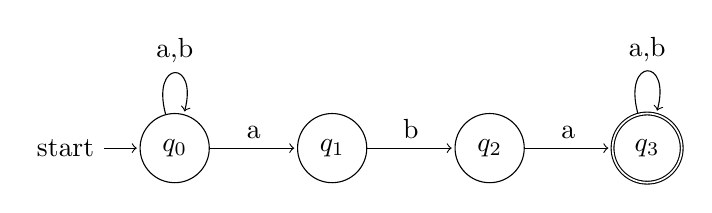
\begin{tikzpicture}[shorten >=1pt,node distance=2cm,on grid,auto] 
   \node[state,initial] (q0) {$q_0$}; 
   \node[state] (q1) [right=of q0] {$q_1$}; 
   \node[state] (q2) [right=of q1] {$q_2$};
   \node[state,accepting] (q3) [right=of q2] {$q_3$};
   
   \path[->] 
    (q0) edge [loop above] node {a,b} (q0)
         edge node {a} (q1)
    (q1) edge node {b} (q2)
    (q2) edge node {a} (q3)
    (q3) edge [loop above] node {a,b} (q3);
\end{tikzpicture}
\caption{Un NFA che riconosce le stringhe che contengono la sottostringa "aba"}
\end{figure}

\begin{errorecomune}
Un errore comune è non sfruttare appieno il non determinismo. Se ti ritrovi con un automa molto complesso, probabilmente non stai utilizzando al meglio le capacità del non determinismo.
\end{errorecomune}

\subsection{Conversione da NFA a DFA: Costruzione per Sottoinsiemi}

\begin{risoluzione}
Per convertire un NFA $N = (Q_N, \Sigma, \delta_N, q_{0_N}, F_N)$ in un DFA equivalente $D = (Q_D, \Sigma, \delta_D, q_{0_D}, F_D)$:

\begin{enumerate}
  \item \textbf{Stati del DFA}: ogni stato del DFA corrisponde a un sottoinsieme degli stati dell'NFA, quindi $Q_D = \powerset(Q_N)$.
  \item \textbf{Stato iniziale}: $q_{0_D} = \{q_{0_N}\}$.
  \item \textbf{Funzione di transizione}: per ogni stato $S \in Q_D$ e simbolo $a \in \Sigma$, definiamo $\delta_D(S, a) = \bigcup_{q \in S} \delta_N(q, a)$.
  \item \textbf{Stati finali}: $F_D = \{S \in Q_D \mid S \cap F_N \neq \emptyset\}$ (cioè, tutti i sottoinsiemi che contengono almeno uno stato finale dell'NFA).
  \item \textbf{Costruzione iterativa}: si parte dallo stato iniziale del DFA e si aggiungono nuovi stati man mano che vengono scoperti tramite le transizioni.
\end{enumerate}
\end{risoluzione}

\begin{suggerimento}
Per gestire la costruzione in modo metodico:
\begin{itemize}
  \item Mantieni una lista di stati del DFA "da elaborare".
  \item Per ogni stato $S$ nella lista, calcola le transizioni per ogni simbolo dell'alfabeto.
  \item Se una transizione porta a un nuovo stato (sottoinsieme) non ancora considerato, aggiungilo alla lista "da elaborare".
  \item Continua finché non ci sono più stati nuovi da elaborare.
\end{itemize}
\end{suggerimento}

\begin{errorecomune}
Un errore comune è non considerare tutti i possibili sottoinsiemi di stati dell'NFA. In pratica, questo succede quando ci si dimentica di calcolare alcune transizioni. È importante tenere traccia degli stati già elaborati e di quelli ancora da elaborare.
\end{errorecomune}

\subsection{$\varepsilon$-NFA e calcolo delle $\varepsilon$-chiusure}

\begin{risoluzione}
Per calcolare l'$\varepsilon$-chiusura di uno stato $q$ in un $\varepsilon$-NFA:

\begin{enumerate}
  \item Inizializza $\eclose{q} = \{q\}$ (uno stato è sempre raggiungibile da sé stesso con zero $\varepsilon$-transizioni).
  \item Per ogni stato $p \in \eclose{q}$, se esiste una $\varepsilon$-transizione da $p$ a un altro stato $r$, aggiungi $r$ a $\eclose{q}$.
  \item Ripeti il passo 2 finché non vengono aggiunti nuovi stati a $\eclose{q}$.
\end{enumerate}

Per convertire un $\varepsilon$-NFA in un NFA senza $\varepsilon$-transizioni:

\begin{enumerate}
  \item Calcola l'$\varepsilon$-chiusura di ogni stato.
  \item Definisci la nuova funzione di transizione $\delta'$ come: $\delta'(q, a) = \bigcup_{p \in \eclose{q}} \eclose{\delta(p, a)}$ per ogni $q \in Q$ e $a \in \Sigma$.
  \item Gli stati finali del nuovo NFA sono tutti gli stati $q$ tali che $\eclose{q} \cap F \neq \emptyset$.
\end{enumerate}
\end{risoluzione}

\begin{suggerimento}
L'$\varepsilon$-chiusura può essere calcolata in modo efficiente utilizzando un algoritmo di ricerca in ampiezza (BFS) o in profondità (DFS) a partire dallo stato iniziale, considerando solo le $\varepsilon$-transizioni.
\end{suggerimento}

\begin{figure}[h]
\centering
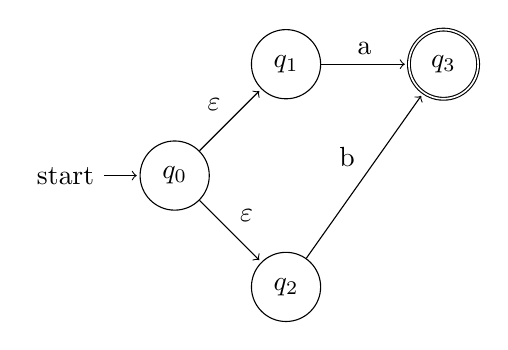
\begin{tikzpicture}[shorten >=1pt,node distance=2cm,on grid,auto] 
   \node[state,initial] (q0) {$q_0$}; 
   \node[state] (q1) [above right=of q0] {$q_1$};
   \node[state] (q2) [below right=of q0] {$q_2$};
   \node[state,accepting] (q3) [right=of q1] {$q_3$};
   
   \path[->] 
    (q0) edge node {$\varepsilon$} (q1)
         edge node {$\varepsilon$} (q2)
    (q1) edge node {a} (q3)
    (q2) edge node {b} (q3);
\end{tikzpicture}
\caption{Un $\varepsilon$-NFA esempio. $\eclose{q_0} = \{q_0, q_1, q_2\}$}
\end{figure}

\begin{errorecomune}
Un errore comune nel calcolo delle $\varepsilon$-chiusure è non considerare le chiusure transitive: se $q$ può raggiungere $p$ con $\varepsilon$-transizioni e $p$ può raggiungere $r$ con $\varepsilon$-transizioni, allora $r$ è nell'$\varepsilon$-chiusura di $q$.
\end{errorecomune}

\subsection{Operazioni su linguaggi regolari}

I linguaggi regolari sono chiusi rispetto a diverse operazioni, e questa proprietà è estremamente utile per la costruzione di automi complessi.

\begin{risoluzione}
Per costruire un automa che riconosca l'unione di due linguaggi regolari $L_1$ e $L_2$:

\begin{enumerate}
  \item Crea un nuovo stato iniziale $q_{new}$.
  \item Aggiungi $\varepsilon$-transizioni da $q_{new}$ agli stati iniziali degli automi per $L_1$ e $L_2$.
  \item L'unione degli stati finali di entrambi gli automi costituisce l'insieme degli stati finali del nuovo automa.
\end{enumerate}

Per costruire un automa che riconosca l'intersezione di due linguaggi regolari $L_1$ e $L_2$:

\begin{enumerate}
  \item Crea il prodotto cartesiano degli stati dei due automi.
  \item Lo stato iniziale è la coppia degli stati iniziali.
  \item Gli stati finali sono tutte le coppie in cui entrambi i componenti sono stati finali.
  \item Per ogni transizione $(q_1, a) \to q_1'$ nel primo automa e $(q_2, a) \to q_2'$ nel secondo, aggiungi una transizione $((q_1, q_2), a) \to (q_1', q_2')$ nell'automa prodotto.
\end{enumerate}

Per costruire un automa che riconosca il complemento di un linguaggio regolare $L$:

\begin{enumerate}
  \item Prendi un DFA che riconosce $L$.
  \item Scambia gli stati finali con quelli non finali (e viceversa).
\end{enumerate}
\end{risoluzione}

\begin{suggerimento}
Per costruire l'automa per operazioni complesse, può essere utile utilizzare costruzioni intermedie. Ad esempio, per $L_1 \setminus L_2$ (differenza), puoi calcolare prima $\overline{L_2}$ (complemento di $L_2$) e poi $L_1 \cap \overline{L_2}$ (intersezione).
\end{suggerimento}

\begin{figure}[h]
\centering
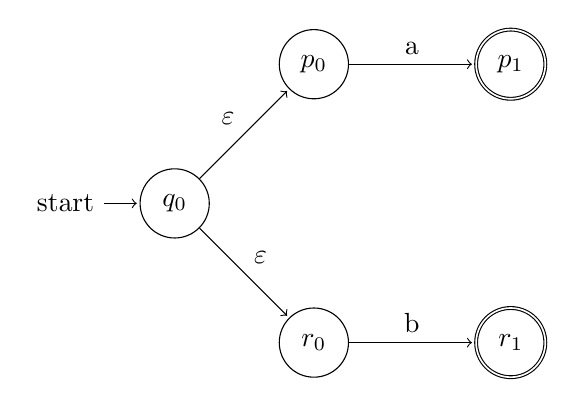
\begin{tikzpicture}[shorten >=1pt,node distance=2.5cm,on grid,auto] 
   \node[state,initial] (q0) {$q_0$}; 
   
   % Automa per L1
   \node[state] (p0) [above right=of q0] {$p_0$}; 
   \node[state,accepting] (p1) [right=of p0] {$p_1$};
   
   % Automa per L2
   \node[state] (r0) [below right=of q0] {$r_0$}; 
   \node[state,accepting] (r1) [right=of r0] {$r_1$};
   
   \path[->] 
    (q0) edge node {$\varepsilon$} (p0)
         edge node {$\varepsilon$} (r0)
    
    % Transizioni per L1
    (p0) edge node {a} (p1)
    
    % Transizioni per L2
    (r0) edge node {b} (r1);
\end{tikzpicture}
\caption{Un NFA che riconosce l'unione di due linguaggi: $L_1 = \{a\}$ e $L_2 = \{b\}$}
\end{figure}

\begin{errorecomune}
Un errore comune è non considerare che il complemento richiede un DFA deterministico. Se si parte da un NFA, è necessario prima convertirlo in un DFA e poi complementare.
\end{errorecomune}

\section{Ricette pratiche per la risoluzione di esercizi tipici}

\subsection{Linguaggi basati su proprietà specifiche}

\begin{enumerate}
  \item \textbf{Stringhe che iniziano con un pattern specifico}:
  \begin{itemize}
    \item Crea un "path" che riconosce il pattern.
    \item Dopo aver riconosciuto il pattern, passa a uno stato che accetta qualsiasi stringa successiva.
  \end{itemize}
  
  \item \textbf{Stringhe che terminano con un pattern specifico}:
  \begin{itemize}
    \item Mantieni un "buffer circolare" di stati che ricorda gli ultimi $n$ simboli, dove $n$ è la lunghezza del pattern.
    \item Lo stato è finale se gli ultimi $n$ simboli corrispondono al pattern.
  \end{itemize}
  
  \item \textbf{Stringhe che contengono un pattern specifico}:
  \begin{itemize}
    \item Usa un NFA con un self-loop sull'inizio per "indovinare" quando inizia il pattern.
    \item Dopo aver riconosciuto il pattern, passa a uno stato finale con self-loop per accettare qualsiasi continuazione.
  \end{itemize}
  
  \item \textbf{Stringhe che non contengono un pattern specifico}:
  \begin{itemize}
    \item Costruisci un DFA che riconosce stringhe che contengono il pattern.
    \item Complementa il DFA (cambiando gli stati finali in non finali e viceversa).
  \end{itemize}
  
  \item \textbf{Stringhe che soddisfano proprietà di conteggio (modulo $n$)}:
  \begin{itemize}
    \item Usa $n$ stati per tenere traccia del conteggio modulo $n$.
    \item Le transizioni aggiornano il conteggio in base al simbolo letto.
  \end{itemize}
\end{enumerate}

\subsection{Interpretazione formale dei linguaggi}

Uno degli aspetti più complessi è tradurre la descrizione informale di un linguaggio in una descrizione formale. Ecco alcune tecniche:

\begin{itemize}
  \item \textbf{Per linguaggi descritti con "inizia con"}: $L = \{w \in \Sigma^* \mid w = xy \text{ dove } x \in S \text{ e } y \in \Sigma^*\}$, dove $S$ è l'insieme dei prefissi validi.
  
  \item \textbf{Per linguaggi descritti con "termina con"}: $L = \{w \in \Sigma^* \mid w = xy \text{ dove } x \in \Sigma^* \text{ e } y \in S\}$, dove $S$ è l'insieme dei suffissi validi.
  
  \item \textbf{Per linguaggi descritti con "contiene"}: $L = \{w \in \Sigma^* \mid w = xyz \text{ dove } x,z \in \Sigma^* \text{ e } y \in S\}$, dove $S$ è l'insieme delle sottostringhe valide.
  
  \item \textbf{Per linguaggi descritti con "non contiene"}: $L = \Sigma^* \setminus \{w \in \Sigma^* \mid w \text{ contiene una sottostringa in } S\}$, dove $S$ è l'insieme delle sottostringhe vietate.
\end{itemize}

\begin{suggerimento}
Quando la descrizione del linguaggio è complessa, cercate di scomporla in condizioni più semplici e poi utilizzate le operazioni sui linguaggi regolari (unione, intersezione, complemento) per combinarle.
\end{suggerimento}

\section{Esempi guidati di risoluzione}

\subsection{Progettazione di un DFA: stringhe che contengono un numero pari di 0}

\begin{risoluzione}
Per riconoscere stringhe che contengono un numero pari di 0 sull'alfabeto $\Sigma = \{0, 1\}$:

\begin{enumerate}
  \item \textbf{Analisi del linguaggio}: dobbiamo contare i simboli 0 modulo 2.
  \item \textbf{Informazione da mantenere}: la parità del numero di 0 letti finora (pari o dispari).
  \item \textbf{Stati}: $q_0$ (numero pari di 0, incluso 0) e $q_1$ (numero dispari di 0).
  \item \textbf{Transizioni}:
    \begin{itemize}
      \item $\delta(q_0, 0) = q_1$ (un 0 in più rende il conteggio dispari)
      \item $\delta(q_0, 1) = q_0$ (1 non influisce sul conteggio di 0)
      \item $\delta(q_1, 0) = q_0$ (un altro 0 rende il conteggio pari)
      \item $\delta(q_1, 1) = q_1$ (1 non influisce sul conteggio di 0)
    \end{itemize}
  \item \textbf{Stato iniziale}: $q_0$ (inizialmente abbiamo letto 0 zeri, che è un numero pari).
  \item \textbf{Stati finali}: $\{q_0\}$ (accettiamo quando il numero di 0 è pari).
\end{enumerate}

\begin{figure}[h]
\centering
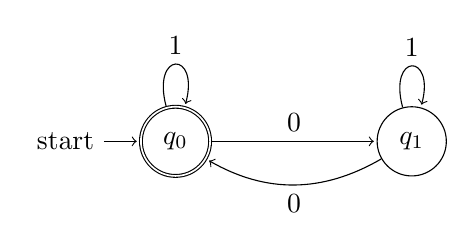
\begin{tikzpicture}[shorten >=1pt,node distance=3cm,on grid,auto] 
   \node[state,initial,accepting] (q0) {$q_0$}; 
   \node[state] (q1) [right=of q0] {$q_1$};
   
   \path[->] 
    (q0) edge node {0} (q1)
         edge [loop above] node {1} (q0)
    (q1) edge [bend left] node {0} (q0)
         edge [loop above] node {1} (q1);
\end{tikzpicture}
\end{figure}
\end{risoluzione}

\subsection{Progettazione di un NFA: stringhe che contengono la sottostringa "aba"}

\begin{risoluzione}
Per riconoscere stringhe che contengono la sottostringa "aba" sull'alfabeto $\Sigma = \{a, b\}$:

\begin{enumerate}
  \item \textbf{Analisi del pattern}: cerchiamo di riconoscere la sequenza esatta "aba".
  \item \textbf{Approccio}: utilizziamo il non determinismo per "indovinare" quando inizia la sottostringa "aba".
  \item \textbf{Stati}:
    \begin{itemize}
      \item $q_0$: stato iniziale, non abbiamo ancora iniziato a riconoscere "aba"
      \item $q_1$: abbiamo riconosciuto "a"
      \item $q_2$: abbiamo riconosciuto "ab"
      \item $q_3$: abbiamo riconosciuto "aba" (stato finale)
    \end{itemize}
  \item \textbf{Transizioni}:
    \begin{itemize}
      \item $\delta(q_0, a) = \{q_0, q_1\}$ (possiamo restare in $q_0$ o iniziare a riconoscere "aba")
      \item $\delta(q_0, b) = \{q_0\}$ (restiamo in $q_0$)
      \item $\delta(q_1, b) = \{q_2\}$ (proseguiamo nel riconoscimento)
      \item $\delta(q_2, a) = \{q_3\}$ (completiamo il riconoscimento)
      \item $\delta(q_3, a) = \{q_3\}$ (resta nello stato finale)
      \item $\delta(q_3, b) = \{q_3\}$ (resta nello stato finale)
    \end{itemize}
  \item \textbf{Stato iniziale}: $q_0$.
  \item \textbf{Stati finali}: $\{q_3\}$.
\end{enumerate}

\begin{figure}[h]
\centering
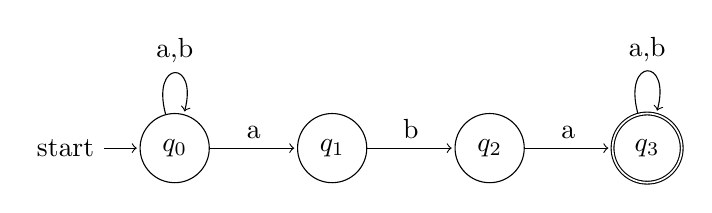
\begin{tikzpicture}[shorten >=1pt,node distance=2cm,on grid,auto] 
   \node[state,initial] (q0) {$q_0$}; 
   \node[state] (q1) [right=of q0] {$q_1$}; 
   \node[state] (q2) [right=of q1] {$q_2$};
   \node[state,accepting] (q3) [right=of q2] {$q_3$};
   
   \path[->] 
    (q0) edge [loop above] node {a,b} (q0)
         edge node {a} (q1)
    (q1) edge node {b} (q2)
    (q2) edge node {a} (q3)
    (q3) edge [loop above] node {a,b} (q3);
\end{tikzpicture}
\end{figure}
\end{risoluzione}

\subsection{Conversione da NFA a DFA mediante sottoinsiemi}

\begin{risoluzione}
Consideriamo il seguente NFA $N$ sull'alfabeto $\Sigma = \{a, b\}$:

\begin{figure}[h]
\centering
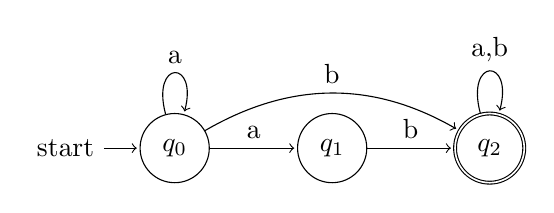
\begin{tikzpicture}[shorten >=1pt,node distance=2cm,on grid,auto] 
   \node[state,initial] (q0) {$q_0$}; 
   \node[state] (q1) [right=of q0] {$q_1$}; 
   \node[state,accepting] (q2) [right=of q1] {$q_2$};
   
   \path[->] 
    (q0) edge [loop above] node {a} (q0)
         edge node {a} (q1)
         edge [bend left] node {b} (q2)
    (q1) edge node {b} (q2)
    (q2) edge [loop above] node {a,b} (q2);
\end{tikzpicture}
\end{figure}

Tabella di transizione dell'NFA:
\begin{center}
\begin{tabular}{c|cc}
 & a & b \\
\hline
$\rightarrow q_0$ & $\{q_0, q_1\}$ & $\{q_2\}$ \\
$q_1$ & $\emptyset$ & $\{q_2\}$ \\
$\ast q_2$ & $\{q_2\}$ & $\{q_2\}$ \\
\end{tabular}
\end{center}

Costruiamo il DFA equivalente:

\begin{enumerate}
  \item \textbf{Stato iniziale del DFA}: $\{q_0\}$
  
  \item \textbf{Calcolo delle transizioni}:
    \begin{itemize}
      \item $\delta_D(\{q_0\}, a) = \delta_N(q_0, a) = \{q_0, q_1\}$
      \item $\delta_D(\{q_0\}, b) = \delta_N(q_0, b) = \{q_2\}$
      \item $\delta_D(\{q_0, q_1\}, a) = \delta_N(q_0, a) \cup \delta_N(q_1, a) = \{q_0, q_1\} \cup \emptyset = \{q_0, q_1\}$
      \item $\delta_D(\{q_0, q_1\}, b) = \delta_N(q_0, b) \cup \delta_N(q_1, b) = \{q_2\} \cup \{q_2\} = \{q_2\}$
      \item $\delta_D(\{q_2\}, a) = \delta_N(q_2, a) = \{q_2\}$
      \item $\delta_D(\{q_2\}, b) = \delta_N(q_2, b) = \{q_2\}$
    \end{itemize}
  
  \item \textbf{Stati finali del DFA}: tutti i sottoinsiemi che contengono $q_2$, quindi $\{q_2\}$.
\end{enumerate}

\begin{figure}[h]
\centering
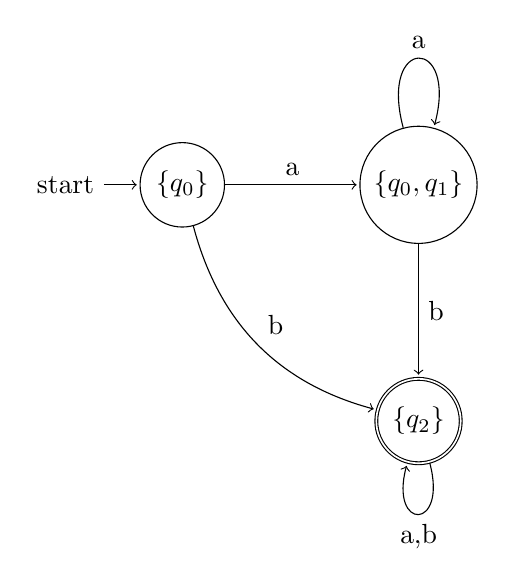
\begin{tikzpicture}[shorten >=1pt,node distance=3cm,on grid,auto] 
   \node[state,initial] (q0) {$\{q_0\}$}; 
   \node[state] (q01) [right=of q0] {$\{q_0, q_1\}$};
   \node[state,accepting] (q2) [below=of q01] {$\{q_2\}$};
   
   \path[->] 
    (q0) edge node {a} (q01)
         edge [bend right] node {b} (q2)
    (q01) edge [loop above] node {a} (q01)
          edge node {b} (q2)
    (q2) edge [loop below] node {a,b} (q2);
\end{tikzpicture}
\end{figure}

Tabella di transizione del DFA risultante:
\begin{center}
\begin{tabular}{c|cc}
 & a & b \\
\hline
$\rightarrow \{q_0\}$ & $\{q_0, q_1\}$ & $\{q_2\}$ \\
$\{q_0, q_1\}$ & $\{q_0, q_1\}$ & $\{q_2\}$ \\
$\ast \{q_2\}$ & $\{q_2\}$ & $\{q_2\}$ \\
\end{tabular}
\end{center}
\end{risoluzione}

\section{Tecniche avanzate di rappresentazione e debugging}

\subsection{Rappresentazione grafica degli automi}

Quando disegnate automi, seguite queste convenzioni:
\begin{itemize}
  \item Lo stato iniziale è indicato con una freccia entrante senza origine.
  \item Gli stati finali sono rappresentati con un doppio cerchio.
  \item Le transizioni sono etichettate con i simboli corrispondenti.
  \item Per chiarezza, le transizioni multiple tra gli stessi stati possono essere combinate (es. "a,b" invece di due frecce separate).
\end{itemize}

\begin{suggerimento}
Nel contesto degli esercizi e degli esami, è importante essere chiari e precisi nei diagrammi. Un buon diagramma può compensare eventuali ambiguità nella descrizione formale.
\end{suggerimento}

\subsection{Debugging degli automi}

Quando un automa non funziona come previsto:
\begin{enumerate}
  \item \textbf{Verifica con esempi semplici}: testa l'automa con stringhe molto semplici (inclusa la stringa vuota).
  \item \textbf{Controlla le transizioni critiche}: verifica che le transizioni per casi speciali siano corrette.
  \item \textbf{Verifica gli stati finali}: assicurati che gli stati finali siano esattamente quelli che dovrebbero essere.
  \item \textbf{Formalizza il linguaggio riconosciuto}: a volte è utile descrivere formalmente il linguaggio che il tuo automa effettivamente riconosce per confrontarlo con quello richiesto.
\end{enumerate}

\begin{suggerimento}
Una tecnica efficace di debugging è eseguire l'automa "a mano" su stringhe di test, tenendo traccia dello stato corrente dopo ogni simbolo letto.
\end{suggerimento}

\section{Errori comuni e come evitarli}

\begin{errorecomune}
\textbf{Confondere NFA e DFA}: in un DFA, per ogni stato e simbolo c'è esattamente una transizione. Se ti ritrovi a scrivere $\delta(q, a) = \{q_1, q_2\}$, stai costruendo un NFA, non un DFA.
\end{errorecomune}

\begin{errorecomune}
\textbf{Transizioni incomplete nei DFA}: ogni stato in un DFA deve avere esattamente una transizione per ogni simbolo dell'alfabeto. Se mancano transizioni, l'automa non è un DFA valido.
\end{errorecomune}

\begin{errorecomune}
\textbf{Errata comprensione dell'$\varepsilon$-chiusura}: l'$\varepsilon$-chiusura include lo stato stesso e tutti gli stati raggiungibili attraverso un qualsiasi numero di $\varepsilon$-transizioni, non solo quelle dirette.
\end{errorecomune}

\begin{errorecomune}
\textbf{Confondere complemento e differenza}: il complemento è rispetto all'universo $\Sigma^*$, mentre la differenza è rispetto a un altro linguaggio specifico. $\overline{L} = \Sigma^* \setminus L$ mentre $L_1 \setminus L_2 = L_1 \cap \overline{L_2}$.
\end{errorecomune}

\
\section{Risorse aggiuntive}

\begin{itemize}
  \item \textbf{JFLAP}: strumento interattivo per la creazione e simulazione di automi, disponibile gratuitamente all'indirizzo \url{http://www.jflap.org/}.
  
  \item \textbf{Simulatori online}:
  \begin{itemize}
    \item \url{https://automata.cs.ru.nl/}
    \item \url{https://ivanzuzak.info/noam/webapps/fsm_simulator/}
  \end{itemize}
  
  \item \textbf{Libri consigliati}:
  \begin{itemize}
    \item Hopcroft, Motwani, Ullman. "Introduction to Automata Theory, Languages, and Computation"
    \item Sipser. "Introduction to the Theory of Computation"
  \end{itemize}
\end{itemize}

\end{document}